\documentclass[utf8]{beamer}
\mode<presentation>
\usepackage[spanish]{babel}
\usepackage{multicol}
\useoutertheme{infolines} 
\usepackage{graphicx}
\usetheme{boxes}

\definecolor{lightblue}{rgb}{0,.5,1}
%\beamertemplateshadingbackground{lightblue!50}{lightblue!50}
%\setbeamercovered{transparent}


\begin{document}
\usebackgroundtemplate{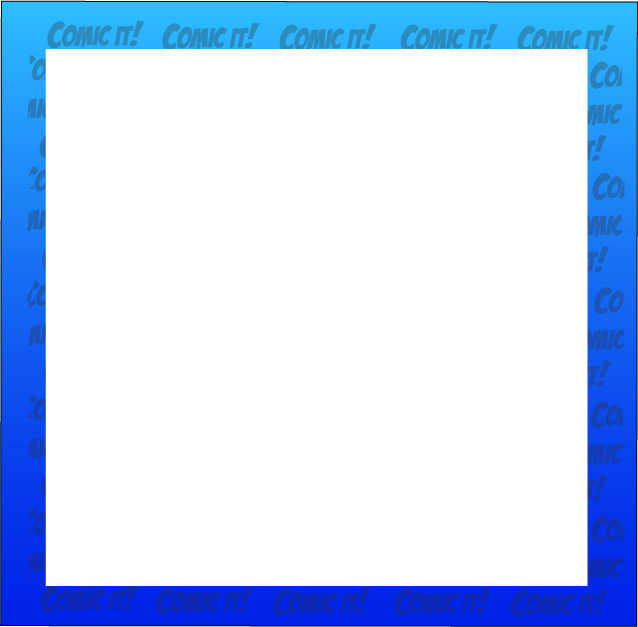
\includegraphics[width= \paperwidth, height=\paperheight]{fondoazul.jpg}}
	\begin{frame}	
		\color{red}\textbf{\begin{center}{\Huge{¡Creando Historietas!}}\end{center}}				
		\pause
		\begin{center} 
				 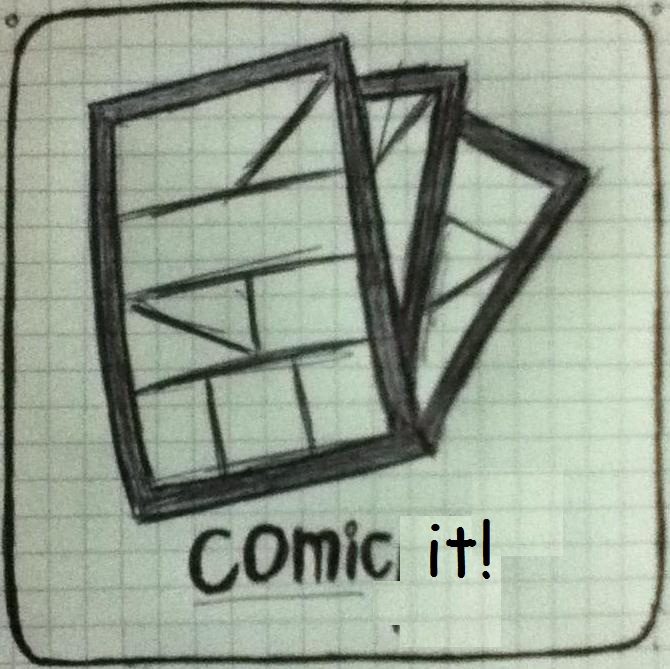
\includegraphics[width=0.5\textwidth]{comicit.jpg} %Midifico el width para cambiar el tamaño%
		\end{center}
	\end{frame}
\usebackgroundtemplate{
\includegraphics[width= \paperwidth, height=\paperheight]{fondoaz.jpg}}
	\begin{frame}	 	
		\color{red}\textbf{\begin{center}{\Huge{Autores}}\end{center}}
		\color{black}
		\begin{center}\huge{ 
			\pause
			- Ana Arias\\
			\pause
			- Liliana Ramos\\
			\pause
			- Denny Schuldt
			
			\pause
		}
			\normalsize
			\vspace{9mm}
			 Lenguajes de Programación
			\\2012 - II Término			
		\end{center}				
	\end{frame}
	\begin{frame}
		\frametitle{
			\begingroup
				\begin{center}
					\color{red}\Huge{Funcionalidades}
				\end{center}
			\endgroup
	 		\begingroup
				\begin{center}
				\normalsize
				\pause
					\color{blue}Haz que tu imagen pase de ser buena...
					\pause
					 ¡A ser increíble!
					\pause
				\end{center}
			\endgroup
		}
		\begin{center}
			\begin{itemize}
				\vspace{-1.5cm}
				\item\textbf{EDICIÓN DE IMAGENES:}
				\newline
				Una opción que permite colocar efectos a la imagen que  desees,
				\newline
				 entre estos efectos tenemos Sepia, Blanco y Negro;  modificar el 
				\newline
				brillo, contraste, entre otras características de la imagen.
			\end{itemize}
		\end{center}
		\begin{center}
			\begingroup
				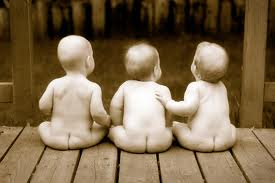
\includegraphics[width=0.25\textwidth]{pic1.jpg}
			\endgroup
			\begingroup
				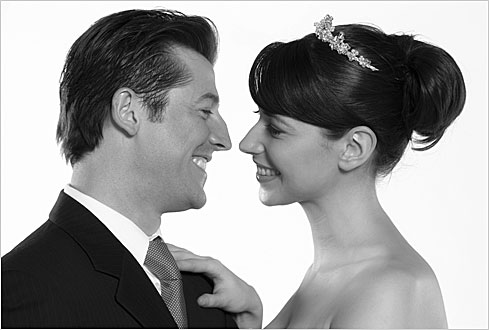
\includegraphics[width=0.25\textwidth]{pic2.jpg}
			\endgroup
			\begingroup
				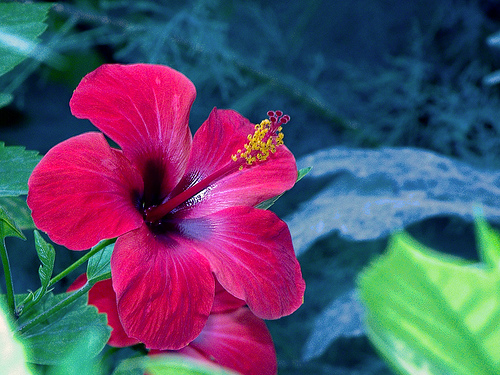
\includegraphics[width=0.25\textwidth]{pic3.jpg}
			\endgroup
		\end{center}
	\end{frame}
	\begin{frame}
		\frametitle{
			\begingroup
				\begin{center}
					\color{red}\Huge{Funcionalidades}
				\end{center}
			\endgroup
	 		\begingroup
				\begin{center}
				\normalsize
				\pause
					\color{blue}¡Crea el diálogo de tus personajes!
					\pause
				\end{center}
			\endgroup
		}
		\begin{center}
			\vspace{-2cm}
			\begin{itemize}
				\item\textbf{LISTA DE BURBUJAS DE DIÁLOGO:}
				\newline
				Proporcionamos una lista con varios formatos de burbujas de
				\newline
				 diálogo, de las cuales el usuario puede escoger las que más  
				\newline
				se ajuste a su necesidad.
				\newline	
				\item\textbf{EDICIÓN DE BURBUJAS DE DIÁLOGO:}
				\newline
				El usuario podrá editar el texto dentro de la burbuja de diálogo 
				\newline
				que haya escogido, con la fuente, tamaño y color que desee.
			\end{itemize}
		\end{center} 
	\end{frame}	
	\begin{frame}
		\begin{center}
			\begin{itemize}
				\vspace{0.5cm}
				\item\textbf{LISTA DE ICONOS:}
				\newline
				Proporcionamos una lista de iconos básicos y personalizados que
				\newline
				 permitirán al usuario crear imágenes más reales y divertidas.
				\newline
				\pause
				\item\textbf{EDICIÓN DE TEXTO O TEXTO PREDETERMINADO:}
				\newline
				Además de íconos, el usuario tendrá una lista de textos divertidos
				\newline
				para darle más creatividad a las escenas que esté creando. Si el u
				\newline
				 suario desea crear nuevos diseños tendrá la opción de hacer sus 
				\newline
				 propios dibujos y colocarlos en la imagen al igual que los iconos.
			\end{itemize}
		\end{center} 
		\pause
		\begin{center}
			\begingroup
				
\includegraphics[width=0.2\textwidth]{icono1.jpg}
			\endgroup
			\pause
			\begingroup
				
\includegraphics[width=0.2\textwidth]{icono2.jpg}
			\endgroup
			\pause
			\begingroup
				
\includegraphics[width=0.2\textwidth]{icono3.jpg}
			\endgroup
		\end{center}
	\end{frame}	
		\begin{frame}
		\frametitle{
			\begingroup
				\begin{center}
					\color{red}\Huge{Funcionalidades}
				\end{center}
			\endgroup
	 		\begingroup
				\begin{center}
				\normalsize
				\pause
					\color{blue}Utiliza las imágenes que acabas de editar!
					\pause
					 ¡Crea tu propia historieta!
					\pause
				\end{center}
			\endgroup
		}
		\begin{center}
			\begin{itemize}
				\vspace{-1.5cm}
				\item\textbf{PLANTILLAS PARA COLOCAR LAS IMAGENES DE LA HISTORIETA:}
				\newline
				Además de poder editar las imágenes, el usuario tendrá la opción 
				\newline
				de crear un collage tipo caricatura con una lista de plantillas que
				\newline
				 les ofrecemos.
				\item\textbf{COLOREAR LAS PLANTILLAS CON PALETAS DE COLORES:}
				\newline
				Después de haber escogido tu plantilla, coloréala con tu color 
				\newline
				favorito, desde una paleta de colores. 
				\newline
				\end{itemize}
		\end{center}
	\end{frame}
	\begin{frame}
		\textbf{
			\newline
			\newline
			\color{red}\hspace{1cm}\huge Ejemplos de plantillas:
		}
		\begin{center} 
			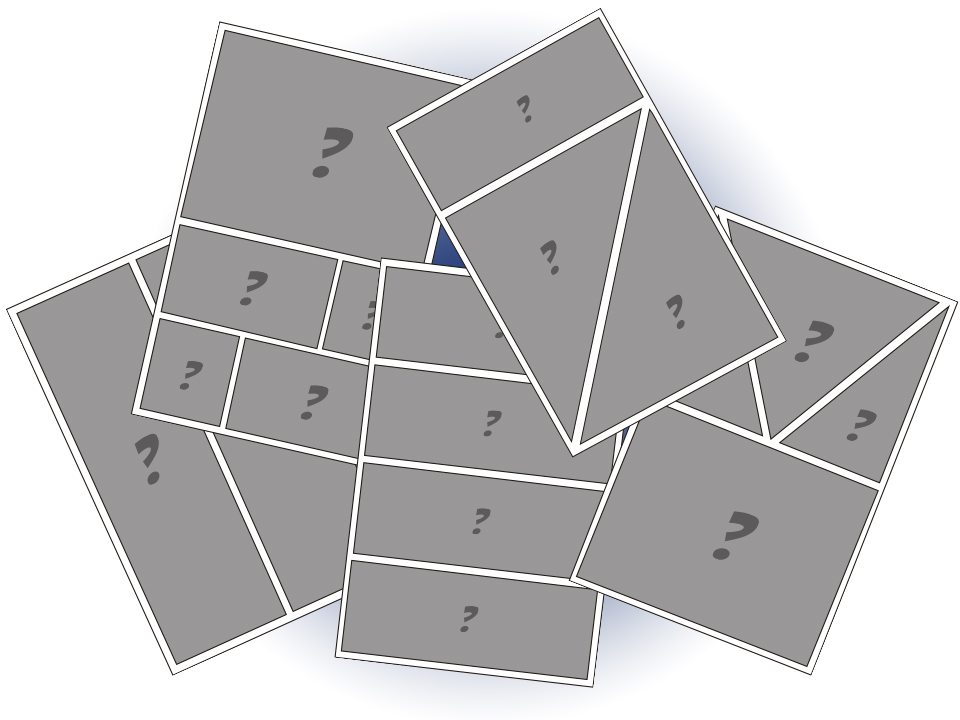
\includegraphics[width=0.75\textwidth]{plantillas.jpg}
		\end{center}
	\end{frame}
	\begin{frame}
		\frametitle{
			\begingroup
				\begin{center}
					\color{red}\Huge{Funcionalidades}
				\end{center}
			\endgroup
	 		\begingroup
				\begin{center}
				\normalsize
				\pause
					\color{blue}¡Cuando termines tu Historieta....
					\pause
					empieza a compartirla!
					\pause
				\end{center}
			\endgroup
		}
		\begin{center}
			\begin{itemize}
				\vspace{-1.5cm}
				\item\textbf{GUARDAR DIBUJO:}
				\newline
				Una vez terminada tu historieta guárdala en el formato que 
				\newline
				desees (.jpg o png).
				\newline
				\item\textbf{COMPARTIR CON FACEBOOK TWITTER:}
				\newline
				Te damos la opción que tu historieta se haga popular entre
				\newline
				 tus amigos al compartirla en redes sociales como Facebook
				\newline
				y Twitter.
				\end{itemize}
		\end{center}
	\end{frame}
		\begin{frame}
		\begin{center} 
			 
\includegraphics[width=0.8\textwidth]{gracias.jpg}
		\end{center}
	\end{frame}
\end{document}

